\noindent{\bf Directions:}
Circle the best answer.

\large




\medskip\hrule
\begin{enumerate}

  \item Interest is the price paid for:
        \begin{enumerate}
          \item Borrowing money
          \item Using money
          \item Saving money
          \item Investing money
        \end{enumerate}

  \item The demand for money comes from:
        \begin{enumerate}
          \item Transactions demand and supply demand
          \item Asset demand and liability demand
          \item Transactions demand and asset demand
          \item Supply demand and asset demand
        \end{enumerate}

  \item According to the Taylor rule, if real GDP rises by 1\% above potential GDP, the Fed should:
        \begin{enumerate}
          \item Lower the Federal funds rate by 0.5 percentage points
          \item Raise the Federal funds rate by 0.5 percentage points
          \item Lower the Federal funds rate by 1 percentage point
          \item Raise the Federal funds rate by 1 percentage point
        \end{enumerate}

        \columnbreak

  \item An expansionary monetary policy involves:
        \begin{enumerate}
          \item Selling bonds, raising the reserve ratio, or raising the discount rate
          \item Buying bonds, raising the reserve ratio, or lowering the discount rate
          \item Selling bonds, lowering the reserve ratio, or raising the discount rate
          \item Buying bonds, lowering the reserve ratio, or lowering the discount rate
        \end{enumerate}

        % \columnbreak


  \item Assume the following:
        \begin{itemize}
          \item The economy's MPC is 0.8
          \item The Fed increases the money supply by \$500 million
        \end{itemize}
        As a result, interest rates decrease, and investment increases
        by \$200 million Calculate the total change in aggregate demand

        \begin{enumerate}
          \item \$200 million
          \item \$500 million
          \item \$800 million
          \item \$1,000 million
        \end{enumerate}

        \columnbreak
        The following information may be helpful in answering the remaining questions:
        \[ i = r^* + \pi^* + a(\pi - \pi^*) + b(y - y^*) \]


  \item Wrap both sides of Taylor's rule with the exponential function; then, compute the Taylor's Series of $e^{ix}$ centered at $x=\pi^*$ and create a polynomial expansion with 4 terms for $e^i$.
        \begin{enumerate}
          \item Selling bonds, raising the reserve ratio, or raising the discount rate
          \item Buying bonds, raising the reserve ratio, or lowering the discount rate
          \item Selling bonds, lowering the reserve ratio, or raising the discount rate
          \item Buying bonds, lowering the reserve ratio, or lowering the discount rate
        \end{enumerate}


  \item In order for Goldman Sachs to most effectively launder
        Malaysia's \textsc{1MDB} sovereign wealth fund, what economic policy
        would be best?
        \begin{enumerate}
          \item Lower the reserve requirement for foreign banks
          \item Increase the reserve requirement for foreign banks
          \item Lower the reserve requirement for domestic banks
          \item Increase the reserve requirement for domestic banks
        \end{enumerate}

  \item If Biden authorizes a \textsc{SWIFT} international banking
        transaction to launder money from Burisma in Ukraine to a hedge
        fund in Washington, D.C., it is an example of which of the
        following types of governmental economic involvement?
        \begin{enumerate}
          \item Open-market operations
          \item Reserve ratio
          \item Discount rate
          \item Government spending
        \end{enumerate}

        \columnbreak
        In 2020, researchers at the University of California, Berkeley
        developed a new margin-based Condorcet voting algorithm called
        Split Cycle, which avoids common pitfalls associated with
        Condorcet voting methods such as ``spoiler effects'' and
        ``strong no show paradoxes''~\cite{splitcycle}.

        \bigskip

        \begin{figure}[h]
          \centering
          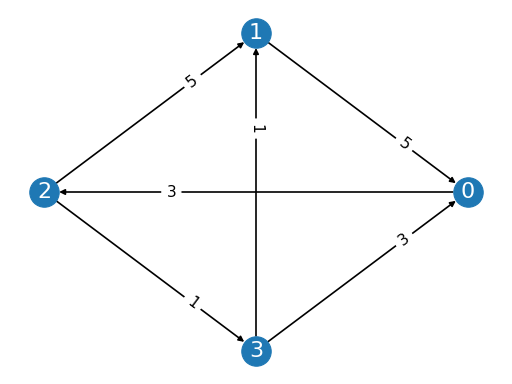
\includegraphics[width=0.4\textwidth]{assets/splitcycle.png}
          \label{fig:example}
          \caption{Voting margins graph}
        \end{figure}

  \item Consider the voting margins matrix above.
        % Define colors for Python syntax highlighting
\definecolor{codegreen}{rgb}{0,0.6,0}
\definecolor{codegray}{rgb}{0.5,0.5,0.5}
\definecolor{codepurple}{rgb}{0.58,0,0.82}
\definecolor{backcolour}{rgb}{0.95,0.95,0.92}

% Define Python language settings
\lstdefinestyle{pythonstyle}{
  backgroundcolor=\color{backcolour},
  commentstyle=\color{codegreen},
  keywordstyle=\color{magenta},
  numberstyle=\tiny\color{codegray},
  stringstyle=\color{codepurple},
  basicstyle=\ttfamily\footnotesize,
  breakatwhitespace=false,
  breaklines=true,
  captionpos=b,
  keepspaces=true,
  numbers=left,
  numbersep=5pt,
  showspaces=false,
  showstringspaces=false,
  showtabs=false,
  tabsize=2
}

\lstset{style=pythonstyle}

\begin{lstlisting}[language=Python, caption=Calling Split Cycle from Python]
from pref_voting.margin_based_methods import split_cycle

split_cycle.display(mg)
\end{lstlisting}


        The above code will run the split cycle algorithm on the margin
        graph. Who will the Condorcet winners be?

        \begin{enumerate}
          \item $\begin{Bmatrix} 2 & 3 \end{Bmatrix}$
          \item $\begin{Bmatrix} 0 & 2 \end{Bmatrix}$
          \item $\begin{Bmatrix} 1 & 3 \end{Bmatrix}$
          \item $\begin{Bmatrix} 2 & 1 \end{Bmatrix}$
        \end{enumerate}
\end{enumerate}